\documentclass[a4j,12pt,]{jarticle}
 \usepackage[dvipdfmx]{graphicx}
 \usepackage{float}
 \usepackage{siunitx} %%SI単位系用
 \usepackage{amssymb, amsmath}
 \usepackage{ascmac,here,txfonts,txfonts}
\usepackage{listings,jlisting}
\usepackage[dvipdfmx]{color}
\lstset{%
  language={Python},
  basicstyle={\small},%
  identifierstyle={\small},%
  commentstyle={\small\itshape\color[rgb]{0,0.5,0}},%
  keywordstyle={\small\bfseries\color[rgb]{0,0,1}},%
  ndkeywordstyle={\small},%
  stringstyle={\small\ttfamily\color[rgb]{1,0,1}},
  frame={tb},
  breaklines=true,
  columns=[l]{fullflexible},%
  numbers=left,%
  xrightmargin=0zw,%
  xleftmargin=3zw,%
  numberstyle={\scriptsize},%
  stepnumber=1,
  numbersep=1zw,%
  lineskip=-0.5ex%
}
\begin{document}

{\noindent\small 第12回報告書 \hfill\today}
\begin{center}
  {\Large 計算値に近い値をとる実測値のみにフィルタリングする処理の実装}
\end{center}
\begin{flushright}
  祖父江匠真 \\
\end{flushright}

\section{はじめに}
前回の報告書より, 相互相関の最大値を計算値のデータ列のリスト長で割った値が, 設定したしきい値を上回るまで再帰的に相互相関の計算に使用する実測データの期間を拡大させることで最適なラグを求める手法は, 事前に実測値と計算値の比を求め, しきい値を下回る比を取る実測値のみにフィルタリングする処理を行う必要があるのではないかという結論に至った.

そこで今回は, 計算値との比を元にフィルタリングした実測値を用いて相互相関を計算することで, 相互相関の最大値に対応するラグが改善するかを確認する下準備として, 実測値を, 計算値に近い値から優先的に指定した割合だけ取得する処理を実装した.

\section{計算値に近いデータをとる実測値を指定した割合だけ取得する処理の実装}
まず, 各日時ごとに実測値と計算値の比を求める.
次に, すべての比について1との差を取り, 絶対値を計算する.
その後, 求めた値を昇順に並び替え, 指定した割合だけ上位から値を取得することで, 実測値を計算値との比をもとにフィルタリングする処理を実装した.

図\ref{p1}から図\ref{p5}に, それぞれ計算値と近い値を取る実測値を上位100\%, 90\%, 80\%, 70\%, 60\%, 50\%になるようフィルタリングした結果を示す.

\begin{figure}[H]
  \begin{center}
    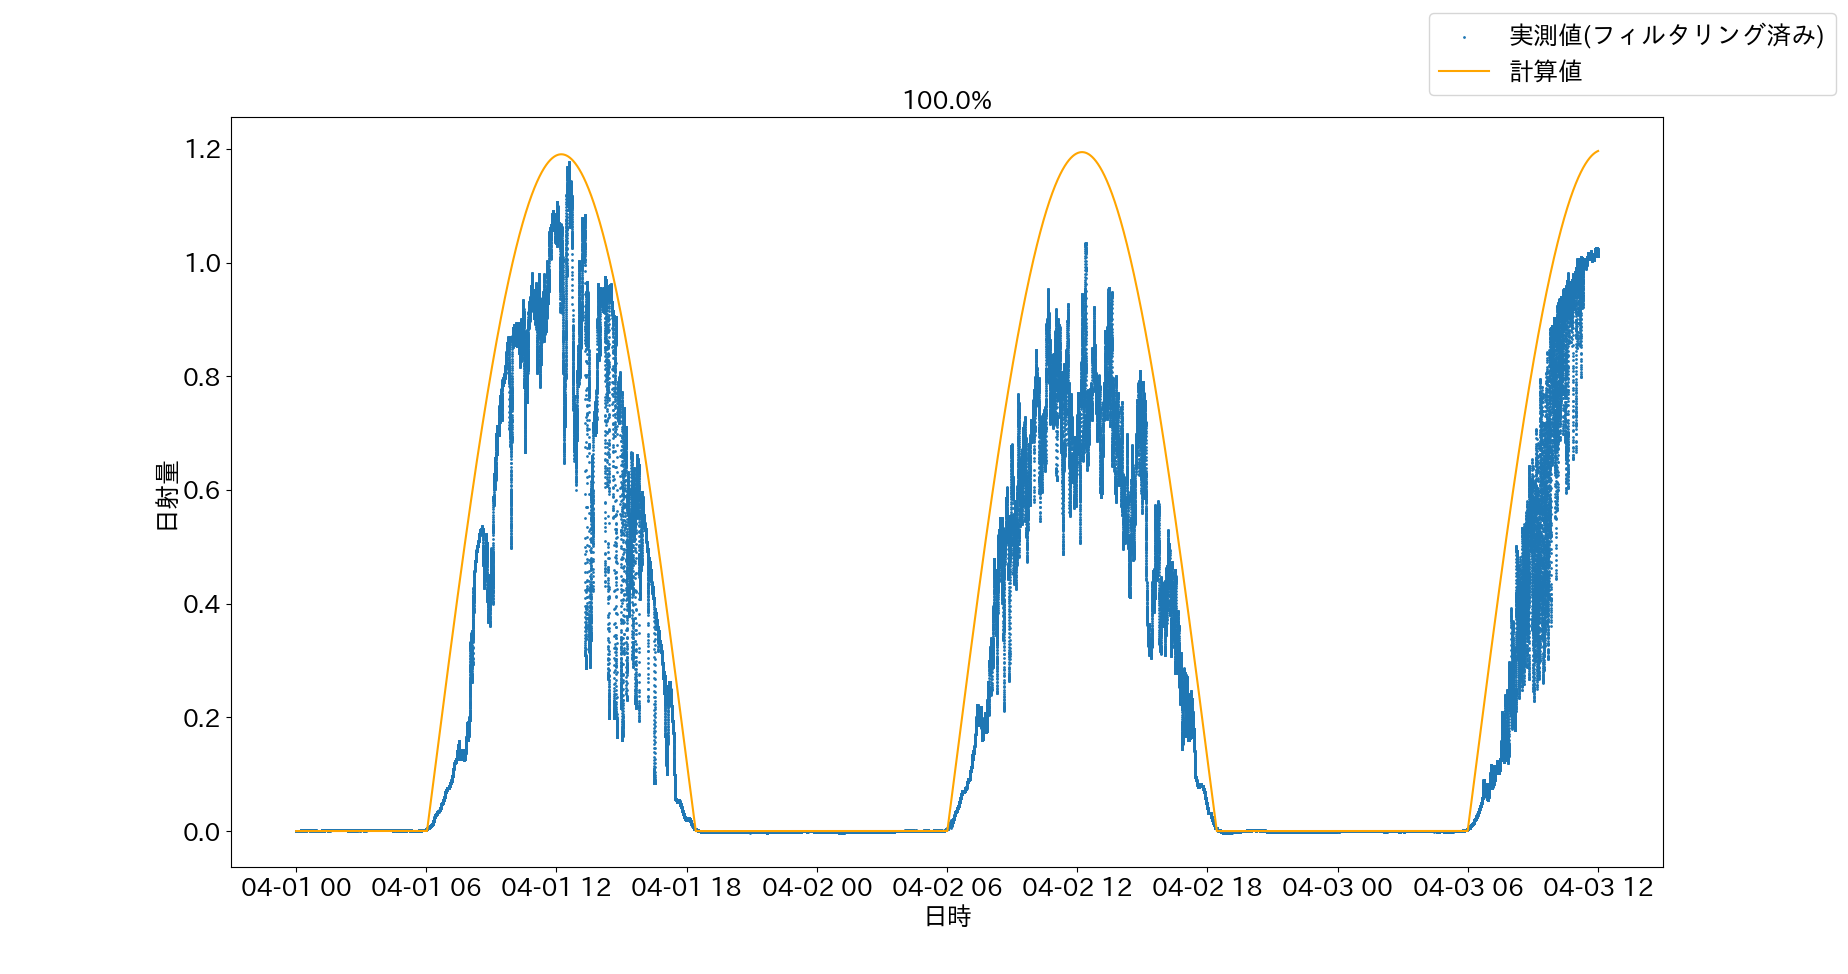
\includegraphics[width=160mm]{100.png}
    \caption{計算値と近い値を取る実測値を上位100\%取得}
    \label{p1}
  \end{center}
\end{figure}

\begin{figure}[H]
  \begin{center}
    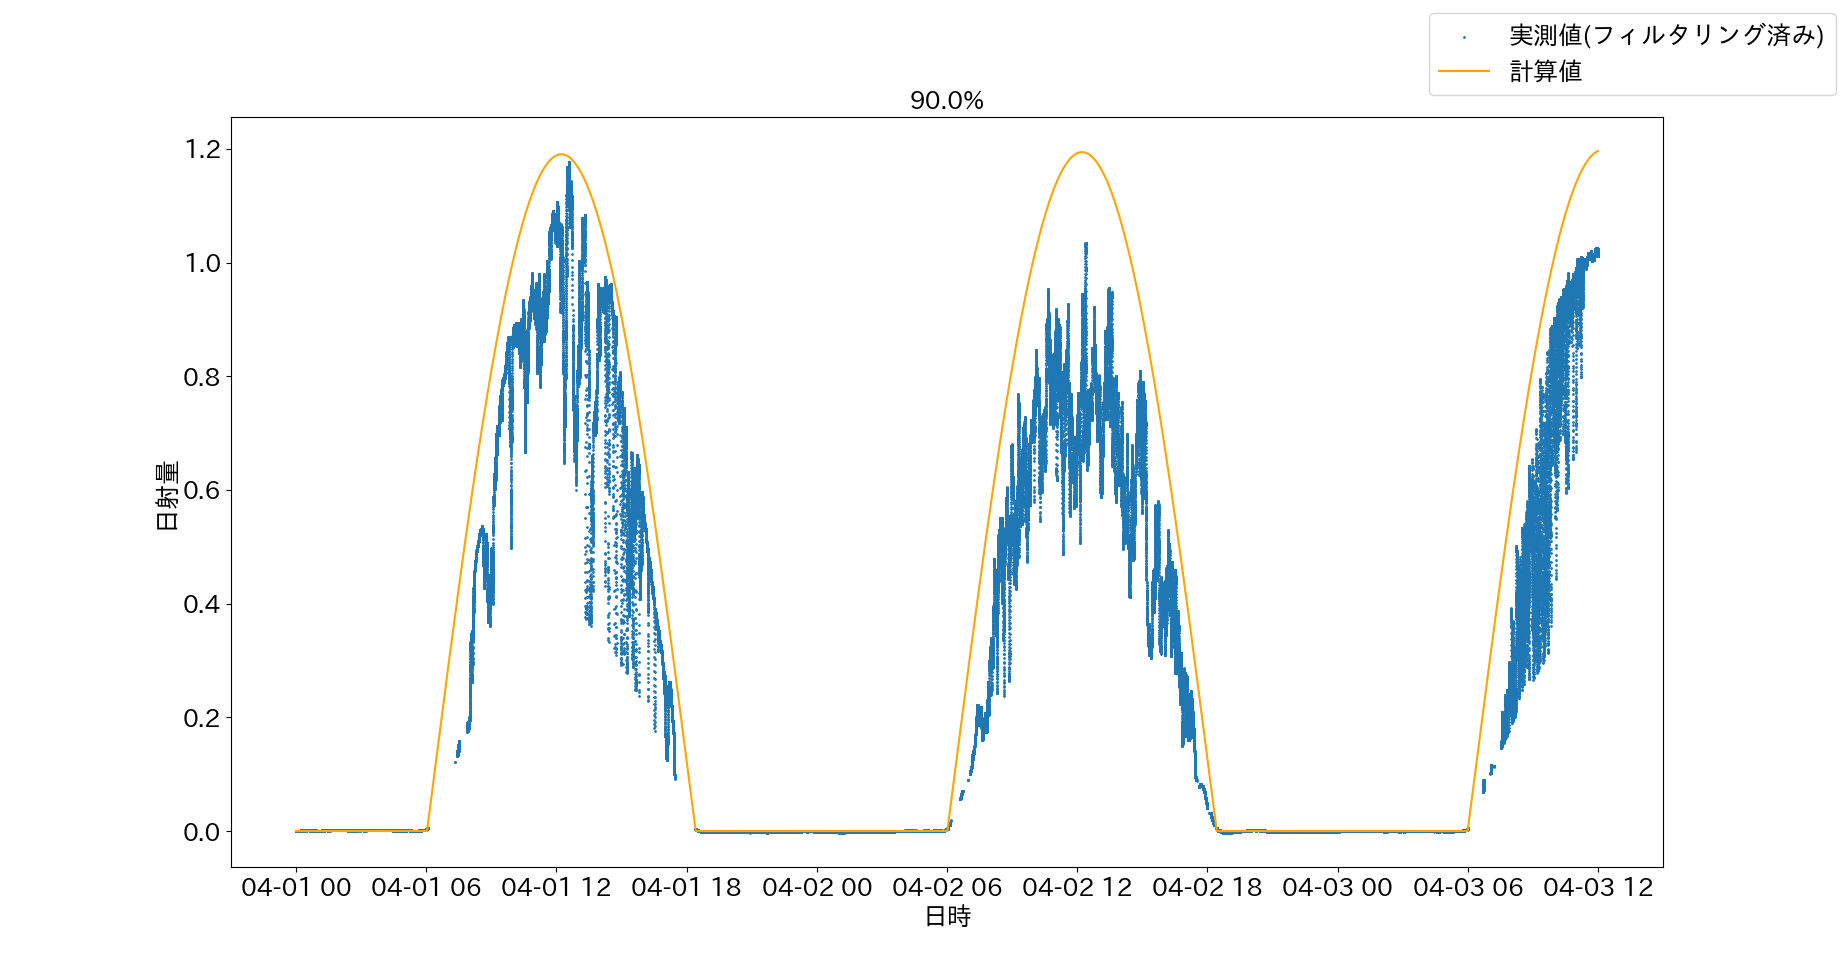
\includegraphics[width=160mm]{90.png}
    \caption{計算値と近い値を取る実測値を上位90\%取得}
    \label{p2}
  \end{center}
\end{figure}

\begin{figure}[H]
  \begin{center}
    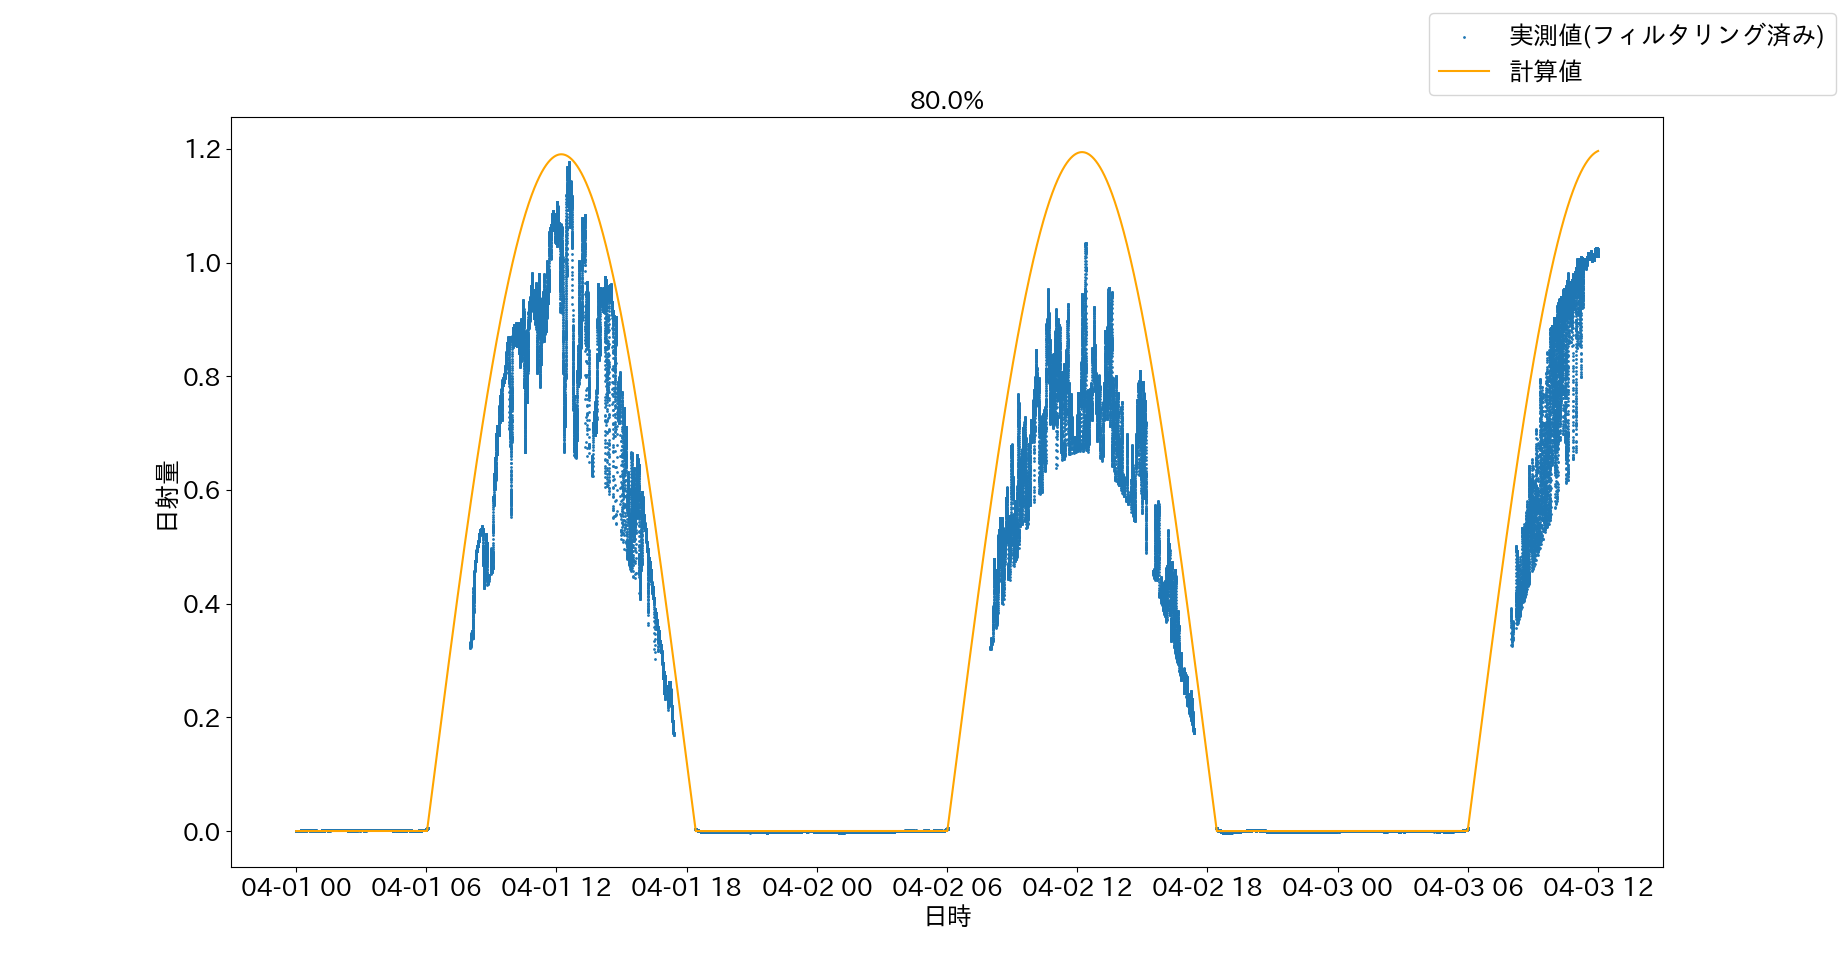
\includegraphics[width=160mm]{80.png}
    \caption{計算値と近い値を取る実測値を上位80\%取得}
    \label{p3}
  \end{center}
\end{figure}

\begin{figure}[H]
  \begin{center}
    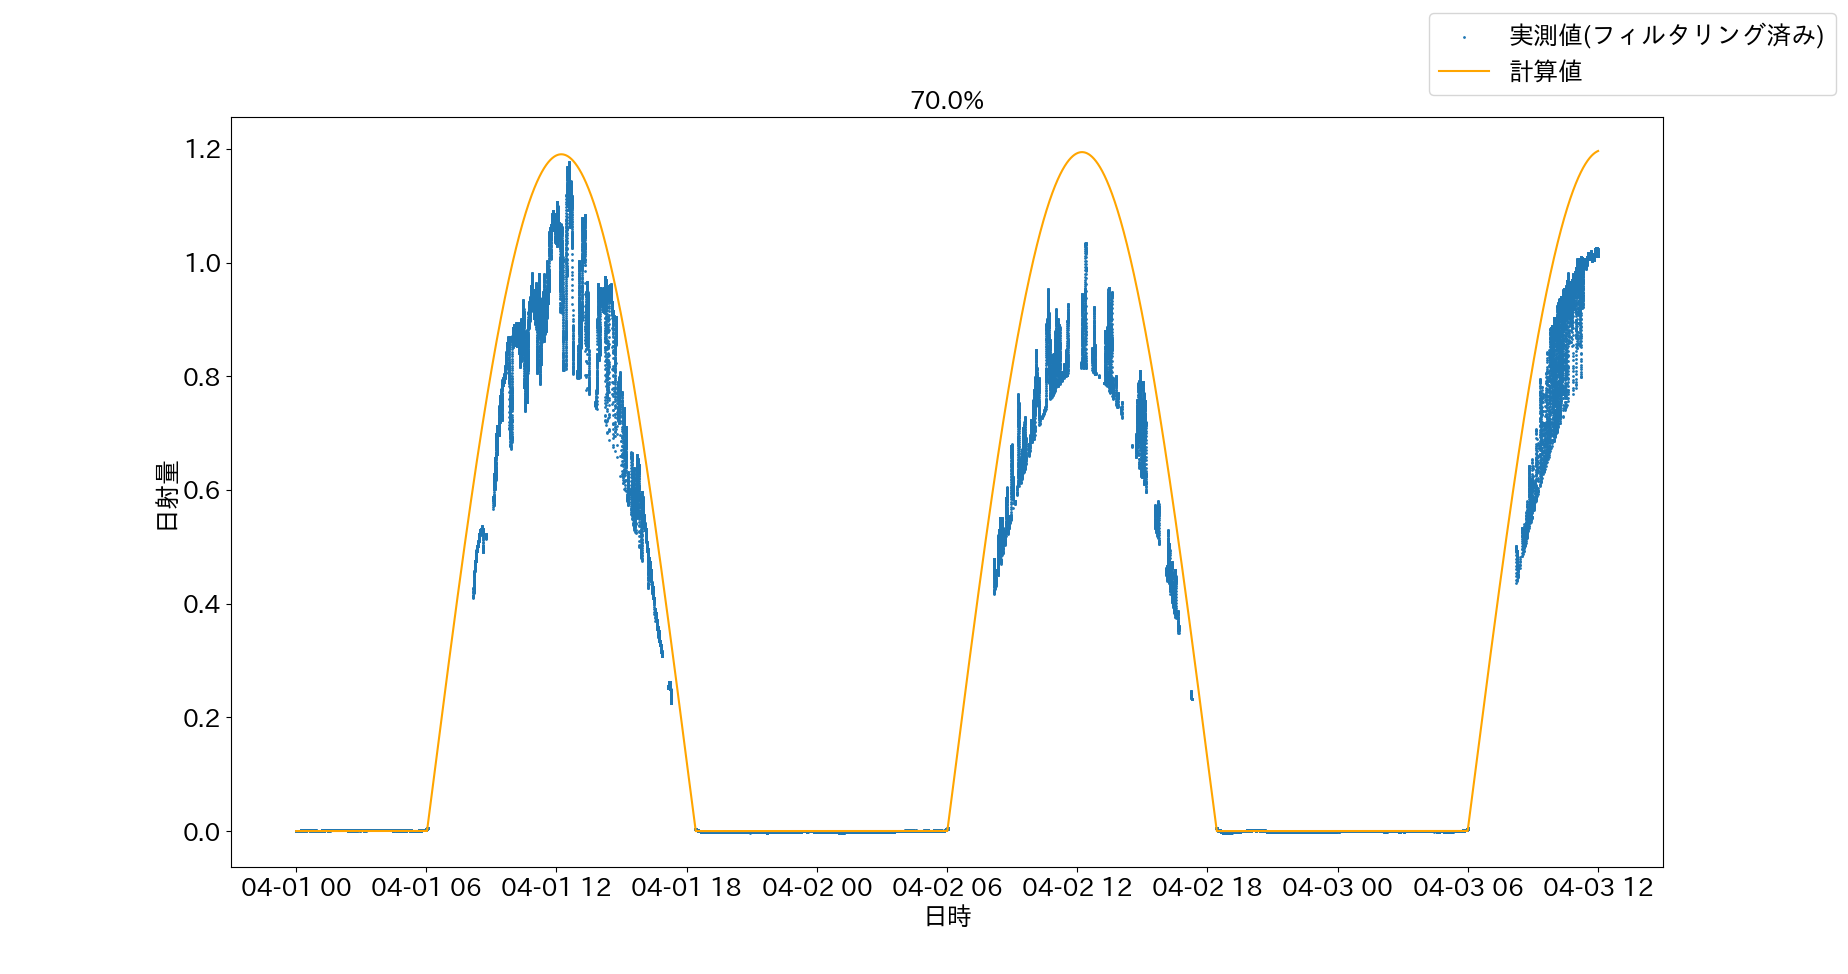
\includegraphics[width=160mm]{70.png}
    \caption{計算値と近い値を取る実測値を上位70\%取得}
    \label{p4}
  \end{center}
\end{figure}

\begin{figure}[H]
  \begin{center}
    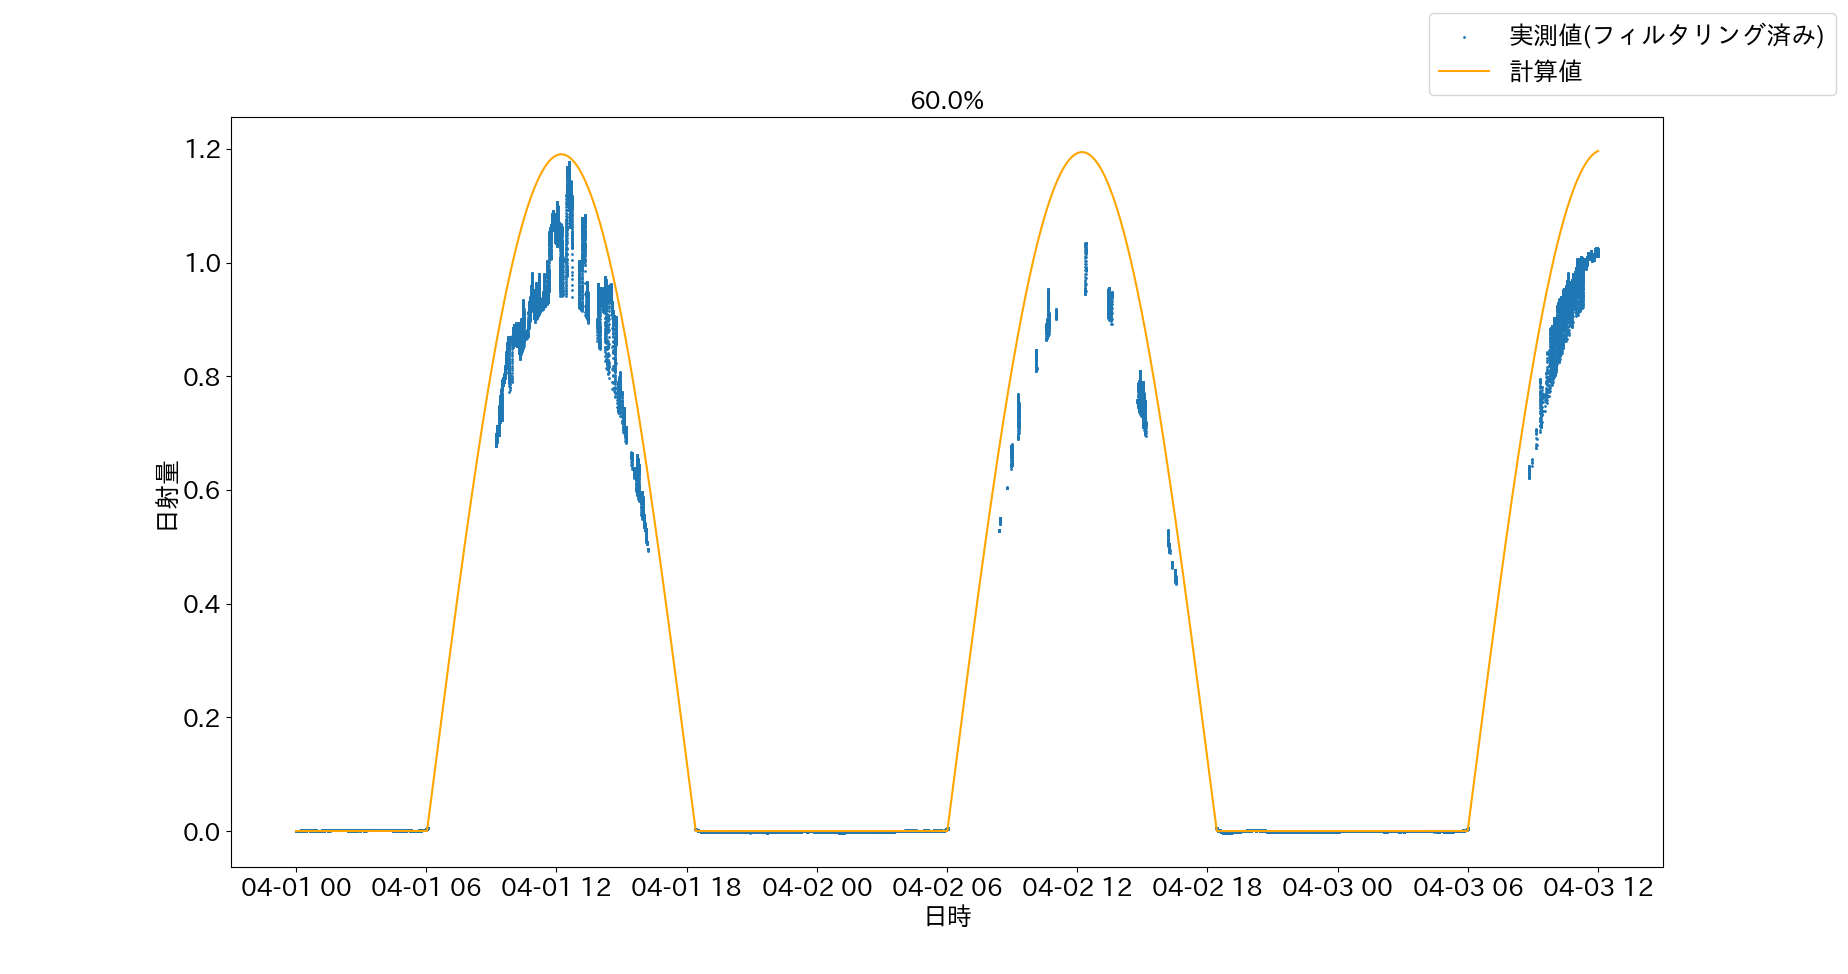
\includegraphics[width=160mm]{60.png}
    \caption{計算値と近い値を取る実測値を上位60\%取得}
    \label{p5}
  \end{center}
\end{figure}

\section{おわりに}
今回は, 実測値を, 計算値に近い値から優先的に指定した割合だけ取得する処理を実装した.

次回は, 今回実装した処理によってフィルタリングした実測値を用いて相互相関を計算することで, 相互相関の最大値に対応するラグが改善するか確認する.

\end{document}